%%%%%%%%%%%%%%%%%%%%%%%%%%%%%%%%%%%%%%%%%%%%%%%%%%%%%%%%%%%%%%%%%%%%%%%%%%%%%%%%%%
%%																				%%
%% File name: 		appendicies.tex												%%
%% Project name:	Hochleistungsantenne										%%
%% Type of work:	T3X00 project work											%%
%% Author:			Sarah Brückner, Maximilian Stiefel, Hannes Bohnengel		%%
%% Date:			13th July 2016												%%
%% University:		DHBW Ravensburg Campus Friedrichshafen						%%
%% Comments:		Created in gedit with tab width = 4							%%
%%																				%%
%%%%%%%%%%%%%%%%%%%%%%%%%%%%%%%%%%%%%%%%%%%%%%%%%%%%%%%%%%%%%%%%%%%%%%%%%%%%%%%%%%

% so that hyperref jumps to the correct position
\phantomsection

% add "Anhang" in toc
\addcontentsline{toc}{chapter}{Anhang}

% start appendicies
\appendix

% to suppress titles of appendices in toc
\addtocontents{toc}{\setcounter{tocdepth}{-1}}

\renewcommand{\thechapter}{Anhang \Alph{chapter}:}

%---------------------------------------------------------------------------------

\chapter{CD}
\label{chap:cdappendix}

\section*{Inhalt}

\begin{itemize}
	\parskip0pt
	\item Studienarbeit: \myemph{T3X00.pdf}
	\item Präsentations-Handout zur Studienarbeit: \myemph{T3X00-Handout.pdf}
	\item Skripte:
	\begin{itemize}
		\item \myemph{rigctld.bat}
		\item \myemph{rigctl.bat}
		\item \myemph{rotctld.bat}
		\item \myemph{rotctl.bat}
		\item \myemph{rigctld-dummy.bat}
		\item \myemph{rotctld-dummy.bat}
	\end{itemize}
	\item Modifizierte Datei: \myemph{gs232.c}
	\item Kompilierter HamLib-Quellcode für Windows: \myemph{hamlib-3.0.1.zip}
\end{itemize}

%---------------------------------------------------------------------------------

\chapter{Skript: \myemph{rigctld.bat}}
\label{chap:rigctldbat}

\begin{center}
	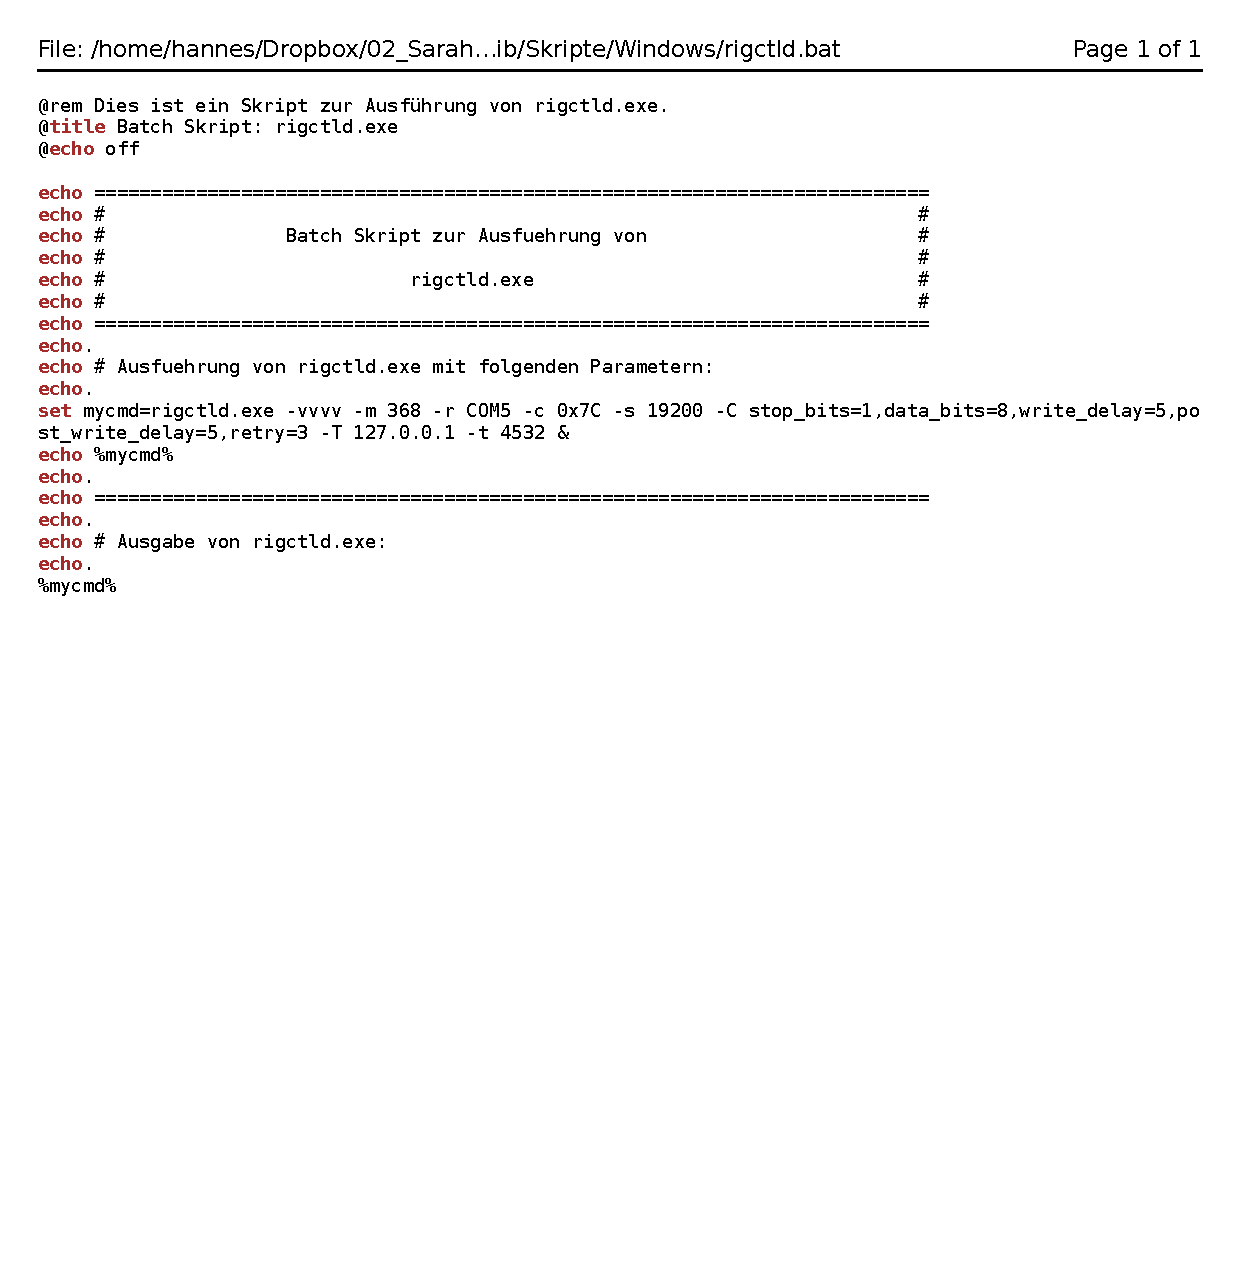
\includegraphics[width=1\textwidth]{./appendicies/rigctld}
\end{center}

%---------------------------------------------------------------------------------

\chapter{Skript: \myemph{rigctl.bat}}
\label{chap:rigctlbat}

\begin{center}
	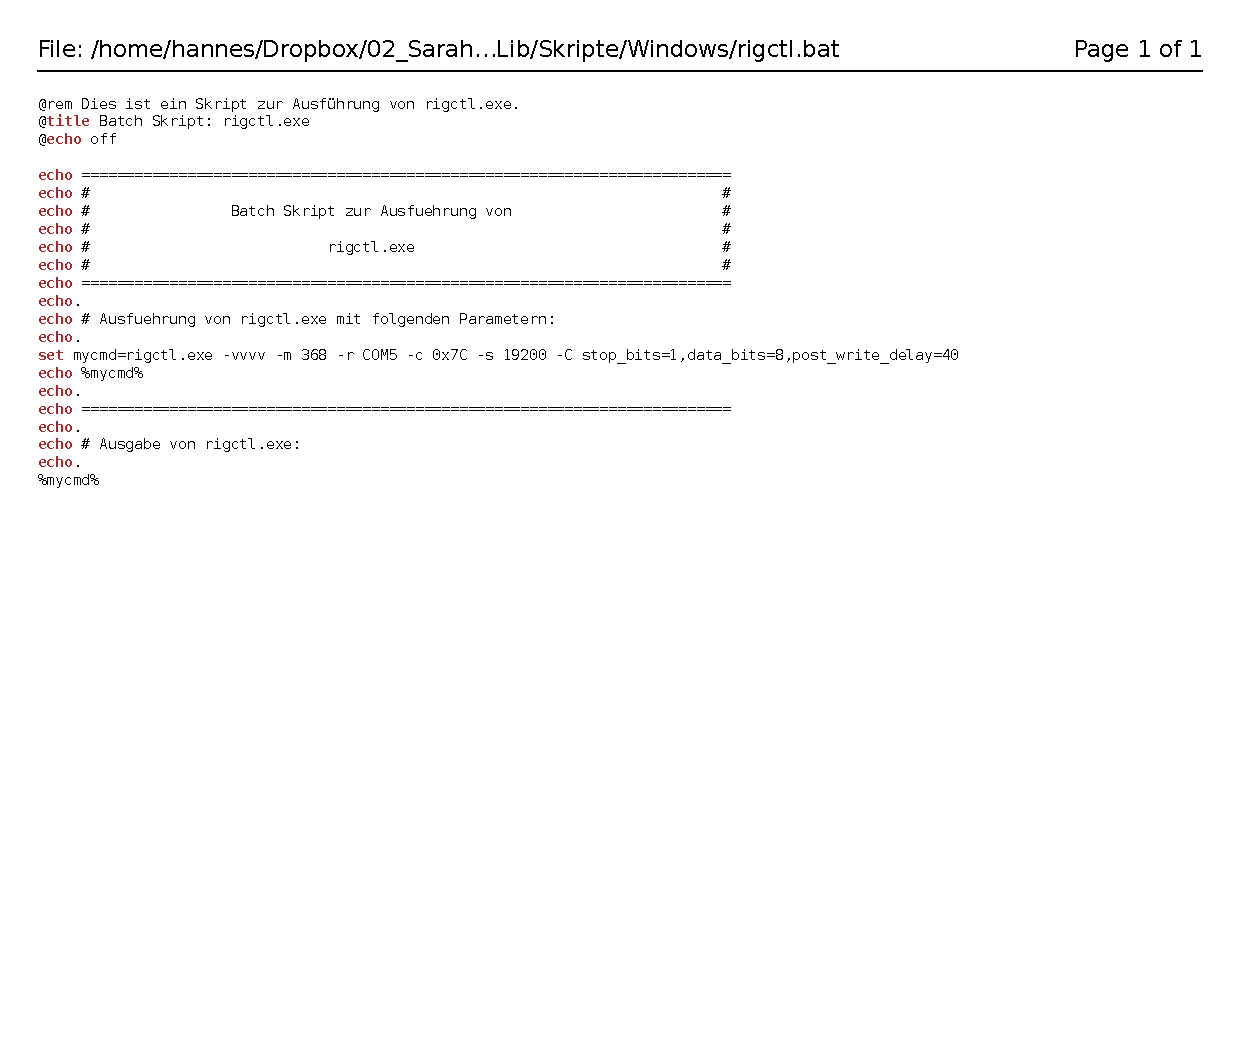
\includegraphics[width=1\textwidth]{./appendicies/rigctl}
\end{center}

%---------------------------------------------------------------------------------

\chapter{Skript: \myemph{rotctld.bat}}
\label{chap:rotctldbat}

\begin{center}
	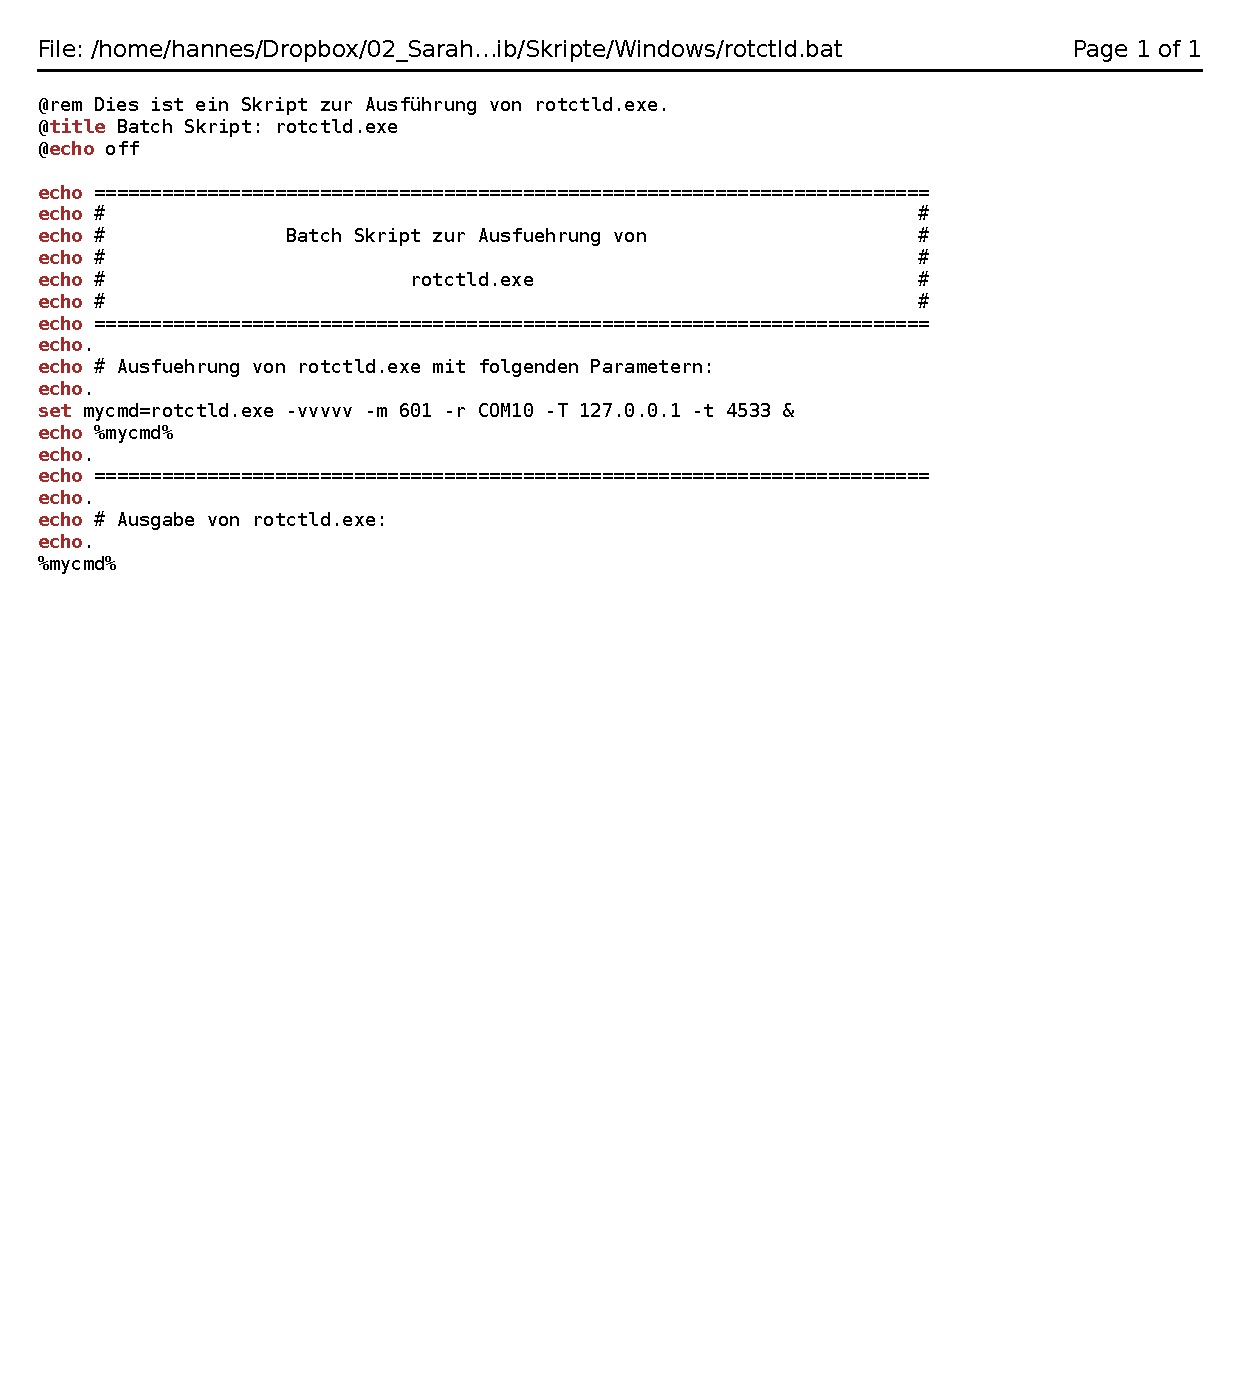
\includegraphics[width=1\textwidth]{./appendicies/rotctld}
\end{center}

%---------------------------------------------------------------------------------

\chapter{Skript: \myemph{rotctl.bat}}
\label{chap:rotctlbat}

\begin{center}
	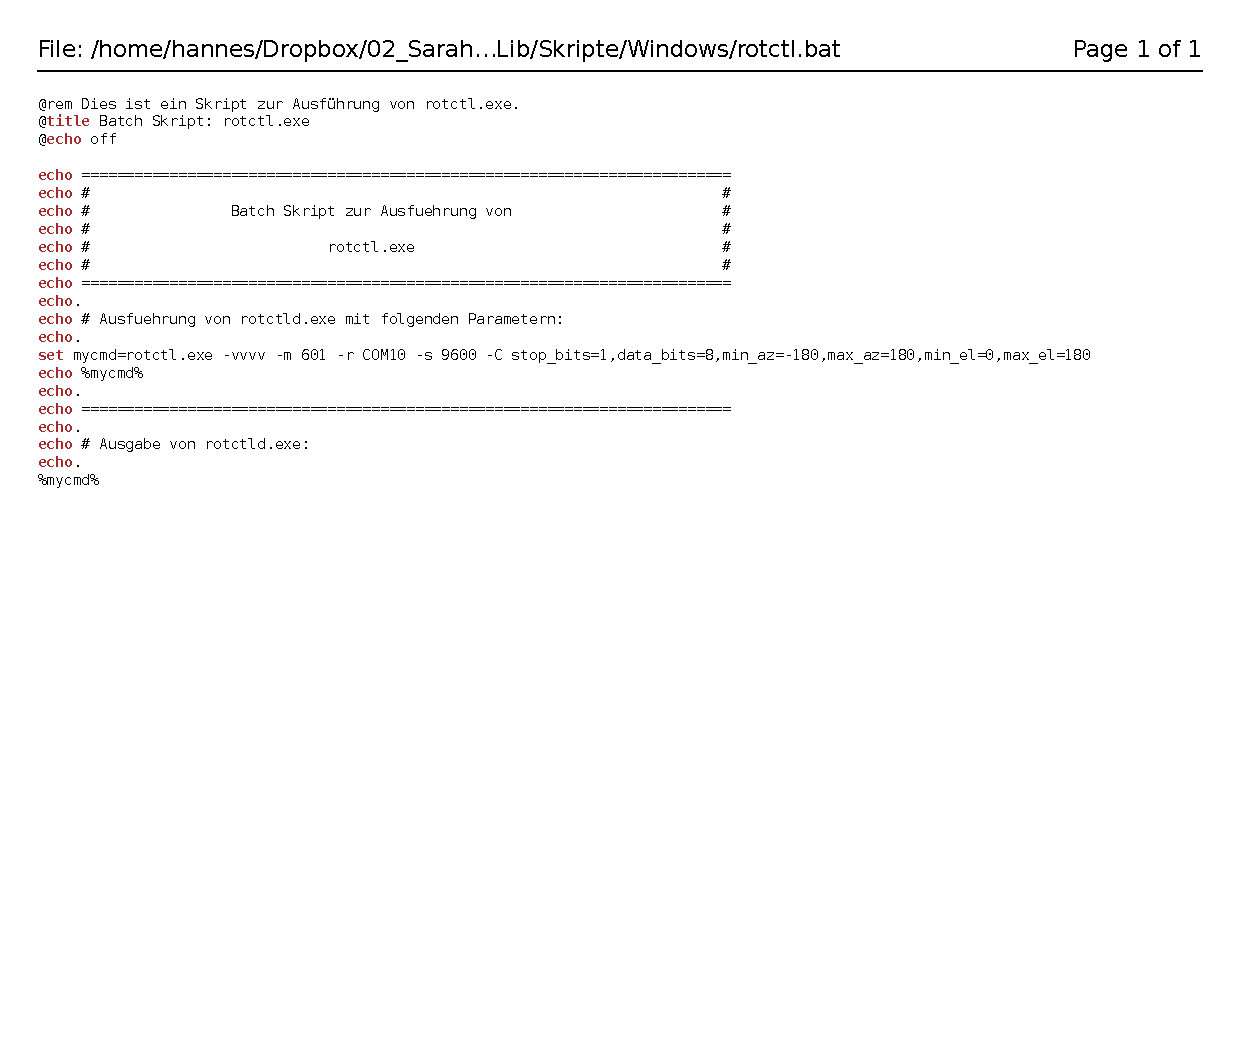
\includegraphics[width=1\textwidth]{./appendicies/rotctl}
\end{center}

%---------------------------------------------------------------------------------

\chapter{Skript: \myemph{rigctld-dummy.bat}}
\label{chap:rigctlddummybat}

\begin{center}
	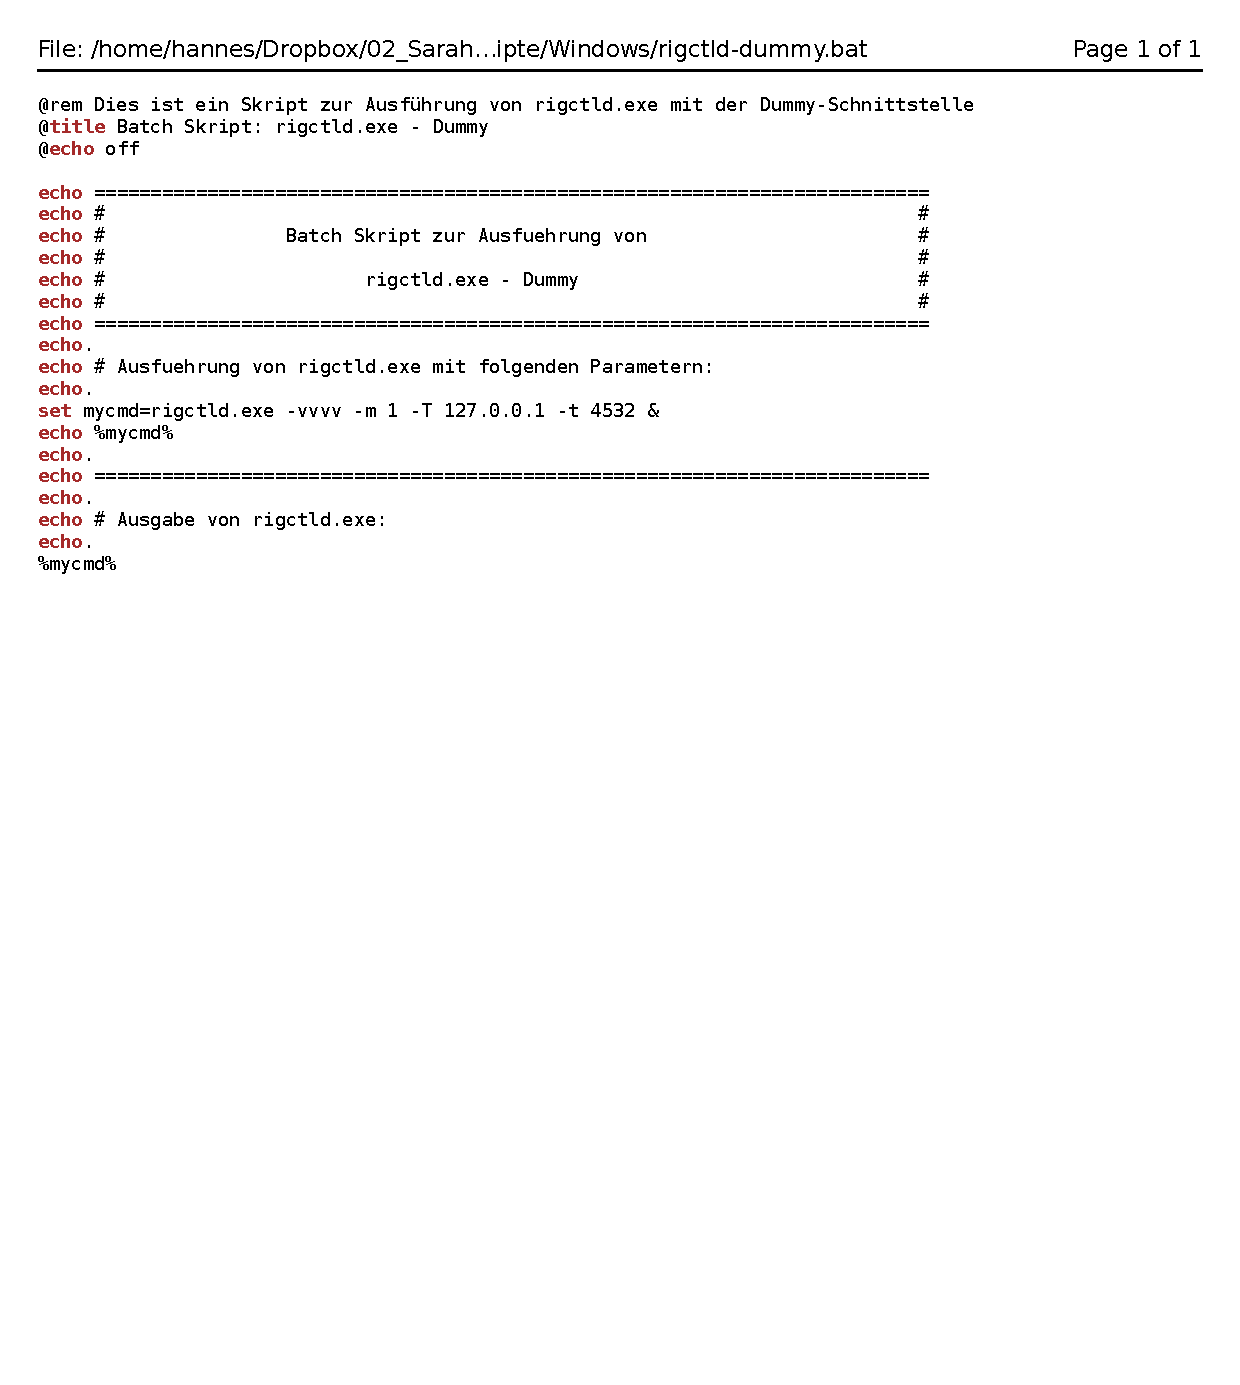
\includegraphics[width=1\textwidth]{./appendicies/rigctld-dummy}
\end{center}

%---------------------------------------------------------------------------------

\chapter{Skript: \myemph{rotctld-dummy.bat}}
\label{chap:rotctlddummybat}

\begin{center}
	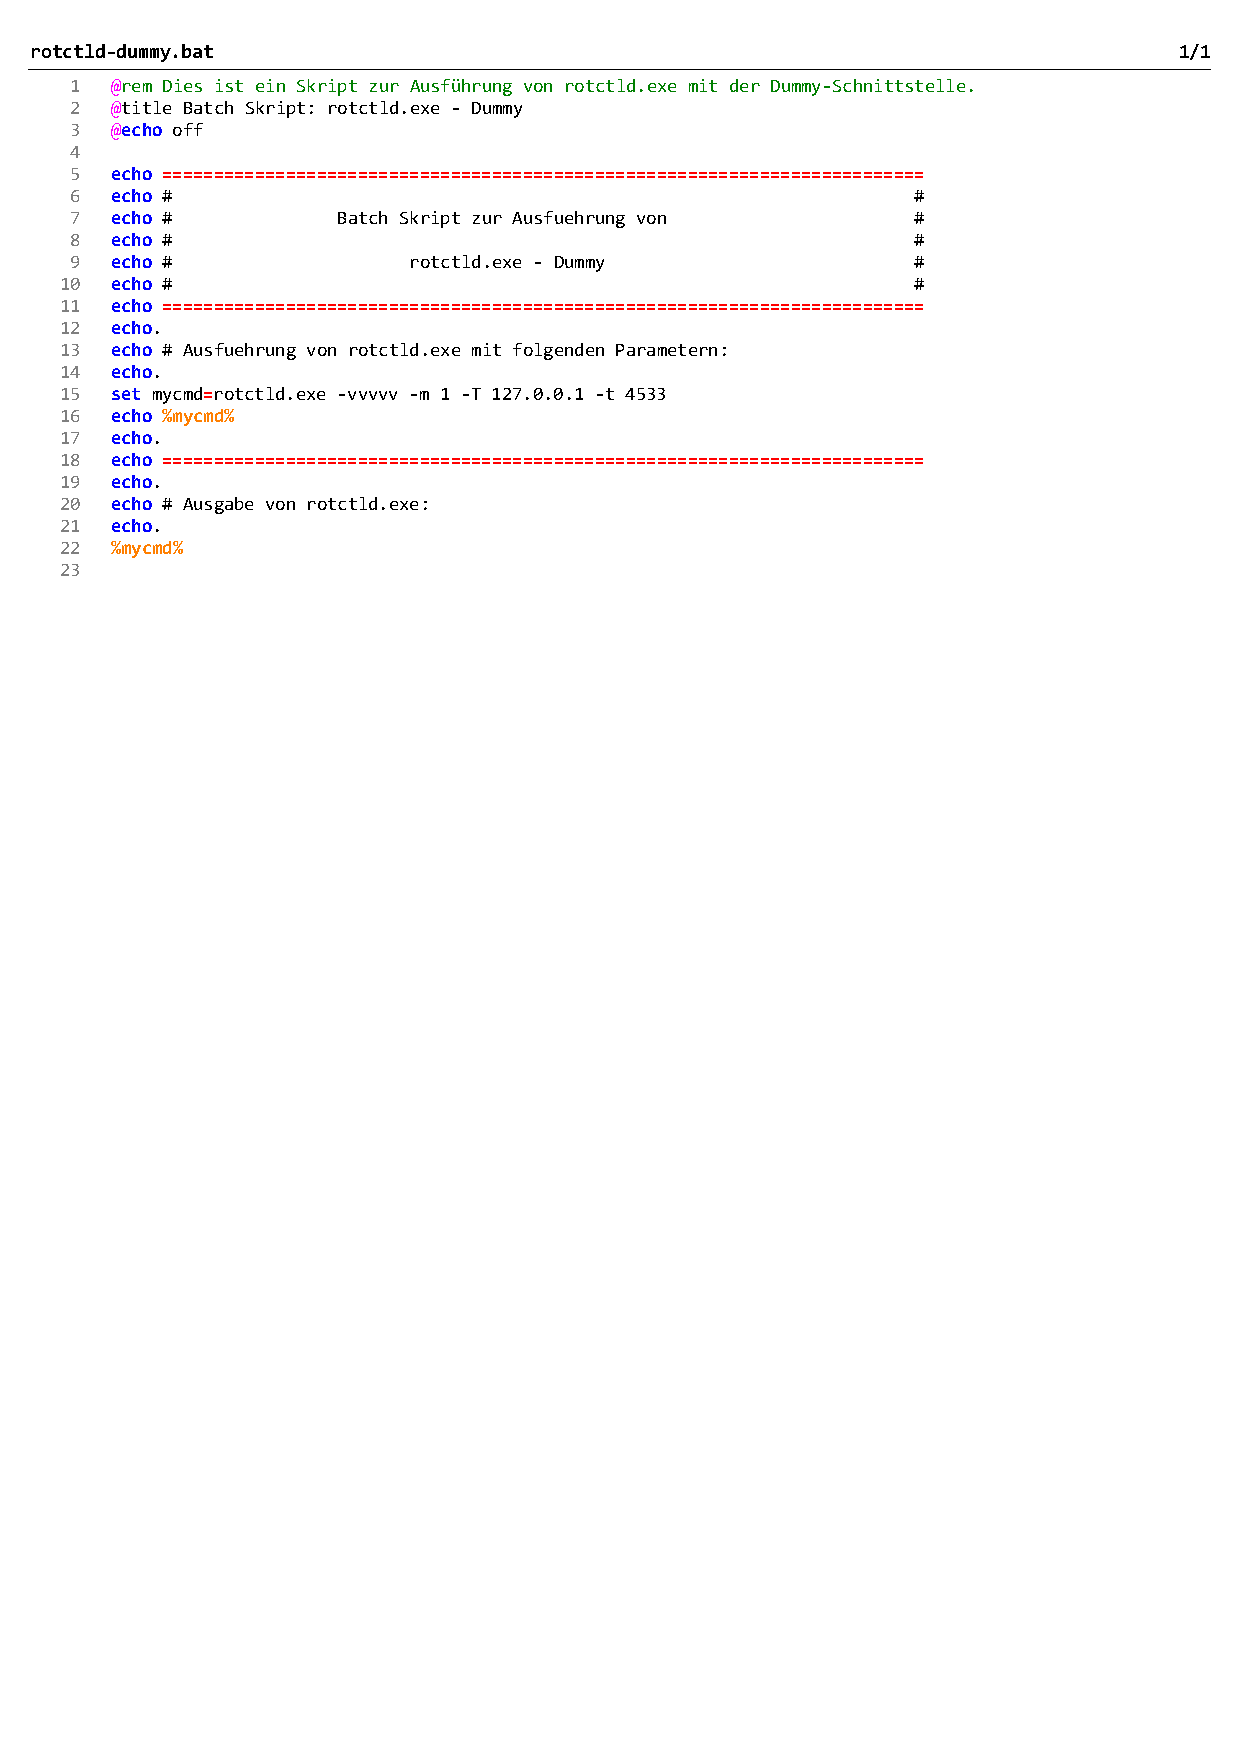
\includegraphics[width=1\textwidth]{./appendicies/rotctld-dummy}
\end{center}

%---------------------------------------------------------------------------------

\chapter{Modifizierte Datei: \myemph{gs232.c}}
\label{chap:hamlibmodification}

\begin{center}
	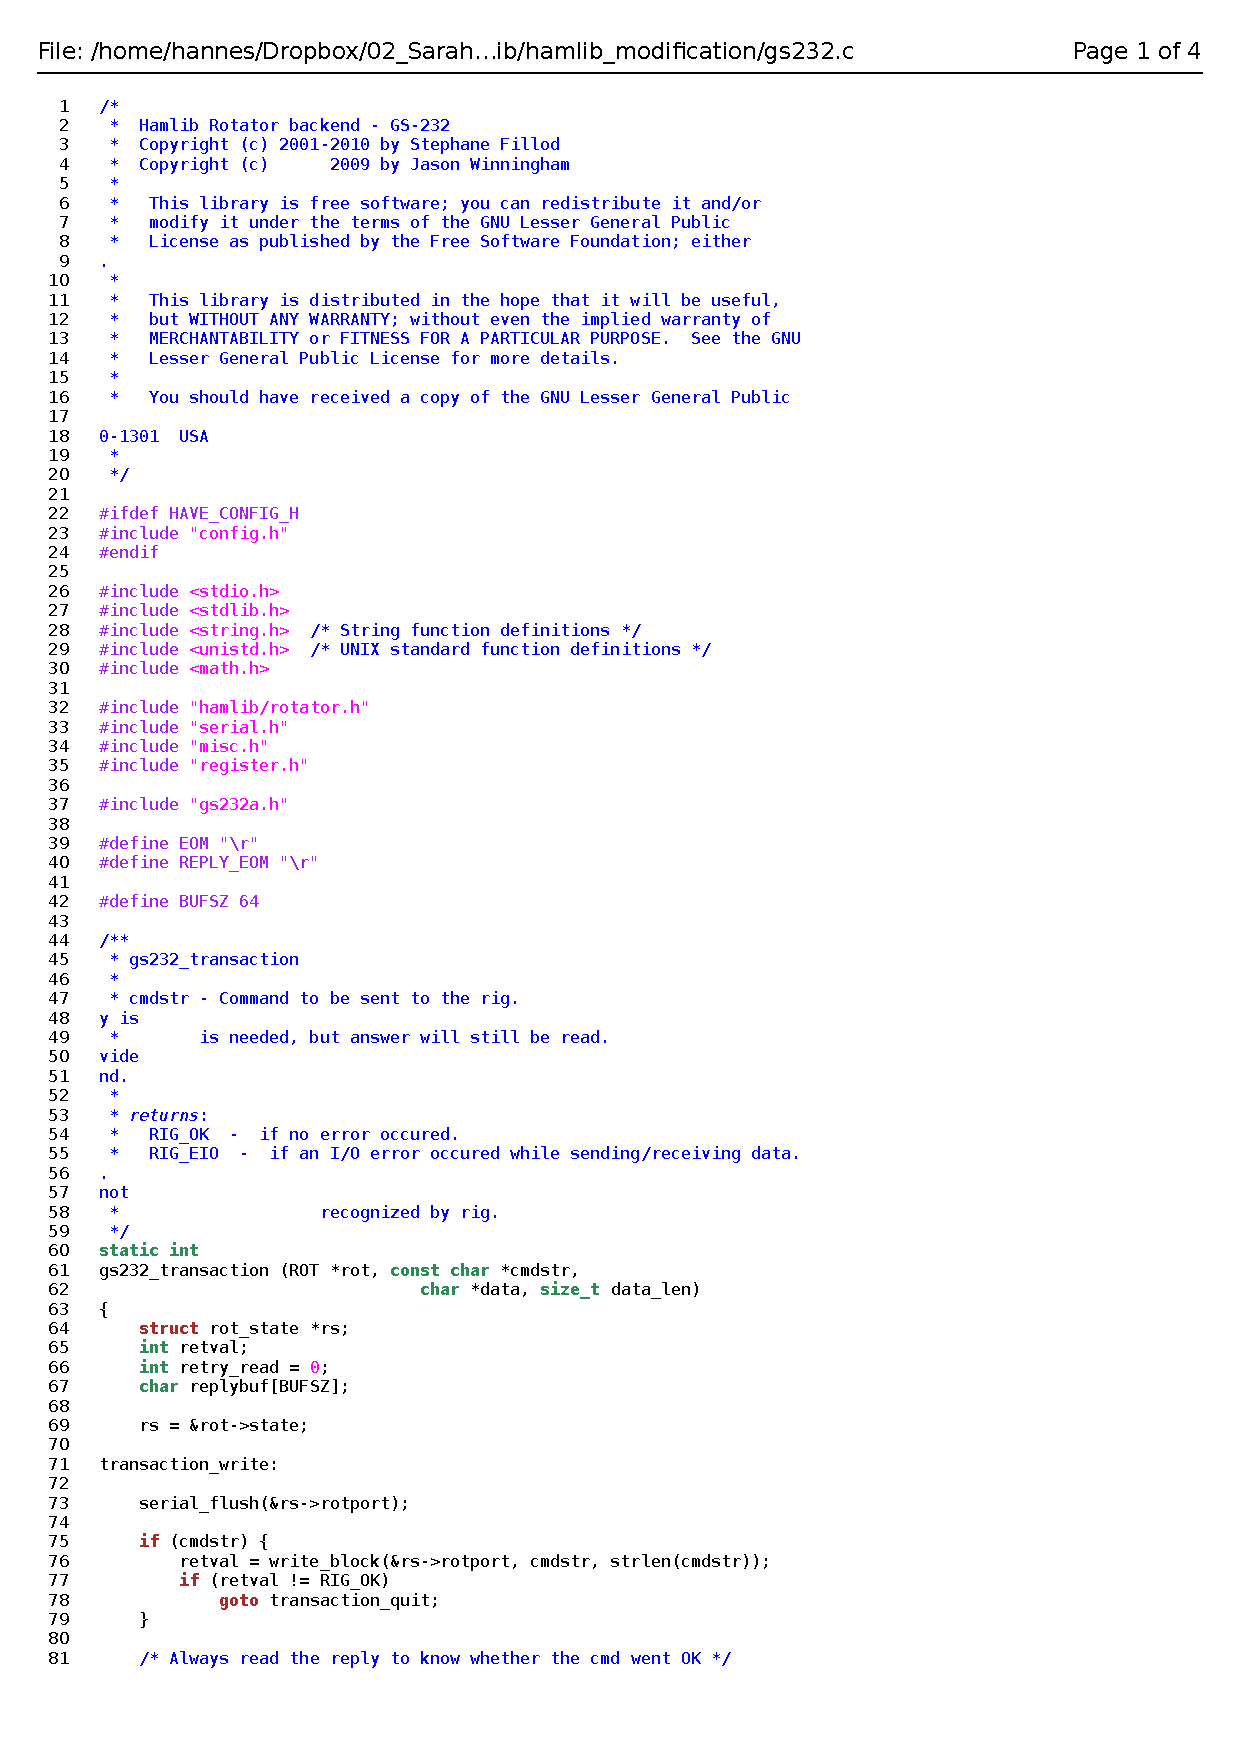
\includegraphics[width=1\textwidth, page=1]{./appendicies/gs232}
\end{center}

\newpage

\begin{center}
	\includegraphics[width=1\textwidth, page=2]{./appendicies/gs232}
\end{center}

\newpage

\begin{center}
	\includegraphics[width=1\textwidth, page=3]{./appendicies/gs232}
\end{center}

\newpage

\begin{center}
	\includegraphics[width=1\textwidth, page=4]{./appendicies/gs232}
\end{center}

%---------------------------------------------------------------------------------